\section{Recursions}

\subsection{Definitions}

$S^1, S^2$ target and query sequences\\
$i_1, j_1, i_2, j_2$ interaction boundaries\\
$si_1, sj_1, si_2, sj_2$ seed boundaries\\
$N$ the maximum interaction length $(\sim 150)$\\
$M$ the enclosed unpaired positions in one loop $(\sim 15)$

General energy computation:

\begin{figure}[H]
	\centering
	\includegraphics[scale=0.45]{seedenergy_general.png}
\end{figure}

\begin{equation*}
E(\substack{i_1,j_1\\i_2,j_2}) = E_{h}^{seed}(\substack{i_1,j_1\\i_2,j_2}) + ED_{1}(\substack{i_1\\j_1}) + ED_{2}(\substack{i_2\\j_2})
\end{equation*}

Optimization task:
\begin{equation*}
\min\limits_{seed}
\min\limits_{\substack{j_{1}-i_{1} \le N\\j_{2}-i_{2} \le N}}
\begin{pmatrix}
E_{h}^{seed}(\substack{i_1,j_1\\i_2,j_2})
\end{pmatrix}\\
\end{equation*}

\subsection{Initialization}

\begin{equation*}
\underset{{\substack{si_1 \le i_{1} \le j_{1} \le sj_{1}\\si_2 \le i_{2} \le j_{2} \le sj_{2}}}}{\forall} E_{h}^{seed}(\substack{i_1,j_1\\i_2,j_2}) = \infty
\end{equation*}

\begin{equation*}
E_{h}^{seed}(\substack{si_1,sj_1\\si_2,sj_2}) = E_{seed}
\end{equation*}

with $E_{seed}$ including $E_{init}$.

\clearpage

\subsection{Recursion 1 ($O(N^{4})$ space + time)}

\begin{figure}[H]
	\centering
	\includegraphics[scale=0.65]{seedenergy.png}
\end{figure}

\begin{equation*}
\substack{
  \underset{\substack{si_{1}-N \le i_{1} \le si_{1}\\si_{2}-N \le i_{2} \le si_{2}}}{\forall}\\
  \underset{\substack{sj_{1} \le j_{1} \le sj_{1}+N\\sj_{2} \le j_{2} \le sj_{2}+N}}{\forall}
}
E_{h}^{seed}(\substack{i_1,j_1\\i_2,j_2}) = \begin{cases}
  \infty\\
  \quad\text{: if } \text{ no matching base pair }\\
  \infty\\
  \quad\text{: if } j_{1} - i_{1} > N \text{ oder } j_{2} - i_{2} > N\\
  \min\limits_{\substack{i_{1} < l_{1} \le r_{1} < j_{1}\\i_{2} < l_{2} \le r_{2} < j_{2}\\l_{1} - i_{1} - 1 \le M\\j_{1}-r_{1}-1 \le M\\l_{2} - i_{2} - 1 \le M\\j_{2}-r_{2}-1 \le M}}
  \begin{pmatrix}
	E_{loop}(\substack{i_1,l_1\\i_2,l_2}) + E_{h}^{seed}(\substack{l_1,r_1\\l_2,r_2}) + E_{loop}(\substack{r_1,j_1\\r_2,j_2})
  \end{pmatrix}\\
  \quad\text{: otherwise.}\\
  
\end{cases}
\end{equation*}

\clearpage

\subsection{Recursion 2 ($O(N^{2})$ space + $O(N^{4})$ time)}

\begin{figure}[H]
	\centering
	\includegraphics[scale=0.65]{seedenergy2.png}
\end{figure}

\begin{equation*}
E_{h}^{seed}(\substack{i_1,j_1\\i_2,j_2}) = \begin{cases}
\infty\\
\quad\text{: if } j_{1} - i_{1} > N \text{ oder } j_{2} - i_{2} > N\\
\begin{pmatrix}
E_{L}(\substack{i_1\\i_2}) + E_{seed} + E_{R}(\substack{j_1\\j_2})
\end{pmatrix}\\
\quad\text{: otherwise.}\\
\end{cases}
\end{equation*}

\begin{equation*}
\underset{\substack{si_{1}-N \le i_{1} \le si_{1}\\si_{2}-N \le i_{2} \le si_{2}}}{\forall}\\
E_L(\substack{i_1\\i_2}) = \begin{cases}
\infty\\
\quad\text{: if } \text{ no matching base pair }\\
\min\limits_{\substack{l_{1} - i_{1} - 1 \le M\\l_{2} - i_{2} - 1 \le M}}
\begin{pmatrix}
E_{loop}(\substack{i_1,l_1\\i_2,l_2}) + E_L(\substack{l_1\\l_2})
\end{pmatrix}\\
\quad\text{: otherwise.}\\

\end{cases}
\end{equation*}

\begin{equation*}
\underset{\substack{sj_{1} \le j_{1} \le sj_{1}+N\\sj_{2} \le j_{2} \le sj_{2}+N}}{\forall}
E_R(\substack{j_1\\j_2}) = \begin{cases}
\infty\\
\quad\text{: if } \text{ no matching base pair }\\
\min\limits_{\substack{j_{1}-r_{1}-1 \le M\\j_{2}-r_{2}-1 \le M}}
\begin{pmatrix}
E_R(\substack{r_1\\r_2}) + E_{loop}(\substack{r_1,j_1\\r_2,j_2})
\end{pmatrix}\\
\quad\text{: otherwise.}\\

\end{cases}
\end{equation*}

\clearpage

\subsection{Recursion 3 ($O(N^{2})$ space + $O(N^{2})$ time)}

First find j1 and j2 that minimize right side. Call them $j_{1opt}$ and $j_{2opt}$. 

\begin{figure}[H]
	\centering
	\includegraphics[scale=0.65]{seedenergy3.png}
\end{figure}

\begin{equation*}
\underset{j1, j2}{\arg\min}
\begin{pmatrix}
E_{seed} + E_{R}(\substack{sj_1,j_1\\sj_2,j_2})
\end{pmatrix}\\
\end{equation*}

with $E_{R}$ defined as in Recursion 2.\\
Then minimize over entire interaction up to $j_{1opt}$ and $j_{2opt}$.

\begin{figure}[H]
	\centering
	\includegraphics[scale=0.65]{seedenergy4.png}
\end{figure}

\begin{equation*}
\underset{\substack{si_{1}-N \le i_{1} \le j_{1}\\si_{2}-N \le i_{2} \le j_{2}}}{\forall}\\
E_{h}^{seed}(\substack{i_1, j_1\\i_2, j_2}) = \begin{cases}
\infty\\
\quad\text{: if } \text{ no matching base pair or $j_1 \neq j_{1opt}$ or $j_2 \neq j_{2opt}$ }\\
\min\limits_{\substack{l_{1} - i_{1} - 1 \le M\\l_{2} - i_{2} - 1 \le M}}
\begin{pmatrix}
E_{loop}(\substack{i_1,l_1\\i_2,l_2}) + E_{L}(\substack{l_1\\l_2}) + E_{seed} + E_{R}(\substack{j_{1opt}\\j_{2opt}})
\end{pmatrix}\\
\quad\text{: otherwise.}\\

\end{cases}
\end{equation*}

with $E_{L}$ and $E_{R}$ defined as in Recursion 2.\\

\clearpage

\subsection{Recursion 4 (ideas from RiBlast2)}

* extend left + right without gaps\\
* extend left + right with gaps\\
* use approximated accessibility energies\\
* ....


